%==============================================================================
% Vampires vs Werewolves AI - Technical Report
% MSc AI - Foundation of AI
% CentraleSupelec 2024-2025
%==============================================================================

\documentclass[11pt,a4paper]{article}

% ============================================================
% PACKAGES
% ============================================================
\usepackage[utf8]{inputenc}
\usepackage[T1]{fontenc}
\usepackage[english]{babel}
\usepackage{geometry}
\usepackage{graphicx}
\usepackage{amsmath,amssymb,amsfonts}
\usepackage{algorithm}
\usepackage{algpseudocode}
\usepackage{listings}
\usepackage{xcolor}
\usepackage{tikz}
\usepackage{pgfplots}
\usepackage{booktabs}
\usepackage{multirow}
\usepackage{hyperref}
\usepackage{caption}
\usepackage{subcaption}
\usepackage{float}
\usepackage{enumitem}
\usepackage{fancyhdr}
\usepackage{titlesec}
\usepackage{tocloft}
\usepackage{pdfpages}
\usepackage{tcolorbox}

% ============================================================
% CONFIGURATION
% ============================================================
\geometry{margin=2.5cm}
\pgfplotsset{compat=1.18}

% TikZ libraries
\usetikzlibrary{shapes.geometric, arrows.meta, positioning, calc, patterns, decorations.pathreplacing, backgrounds, fit, matrix}

% Code listing style
\lstdefinestyle{pythonstyle}{
    language=Python,
    basicstyle=\ttfamily\footnotesize,
    keywordstyle=\color{blue}\bfseries,
    commentstyle=\color{gray}\itshape,
    stringstyle=\color{orange},
    numbers=left,
    numberstyle=\tiny\color{gray},
    numbersep=8pt,
    breaklines=true,
    showstringspaces=false,
    frame=single,
    framerule=0.5pt,
    rulecolor=\color{gray!50},
    backgroundcolor=\color{gray!5},
    tabsize=4,
}
\lstset{style=pythonstyle}

% Hyperref configuration
\hypersetup{
    colorlinks=true,
    linkcolor=blue!60!black,
    citecolor=green!50!black,
    urlcolor=blue!70!black,
    pdftitle={Vampires vs Werewolves AI - Technical Report},
    pdfauthor={MSc AI Team},
}

% Header/Footer
\pagestyle{fancy}
\fancyhf{}
\fancyhead[L]{\footnotesize Vampires vs Werewolves AI}
\fancyhead[R]{\footnotesize MSc AI - Foundation of AI}
\fancyfoot[C]{\thepage}
\renewcommand{\headrulewidth}{0.4pt}

% Custom colors
\definecolor{vampireRed}{RGB}{139, 0, 0}
\definecolor{werewolfBlue}{RGB}{25, 25, 112}
\definecolor{humanGreen}{RGB}{34, 139, 34}
\definecolor{criticalRed}{RGB}{220, 20, 60}
\definecolor{warningOrange}{RGB}{255, 140, 0}

% ============================================================
% TITLE PAGE
% ============================================================
\begin{document}

\begin{titlepage}
    \centering
    \vspace*{1cm}

    {\scshape\LARGE CentraleSup\'elec \par}
    \vspace{0.5cm}
    {\scshape\Large MSc Artificial Intelligence\par}
    {\scshape\large Foundation of Artificial Intelligence\par}
    \vspace{2cm}

    \rule{\textwidth}{1.5pt}\par
    \vspace{0.7cm}
    {\Huge\bfseries Vampires vs Werewolves\\[0.3cm] Adversarial Game AI\par}
    \vspace{0.5cm}
    \rule{\textwidth}{1.5pt}\par

    \vspace{1.5cm}

    {\Large\itshape Technical Report\\[0.2cm]
    Alpha-Beta Pruning with Iterative Deepening\par}

    \vspace{2cm}

    % Architecture diagram preview
    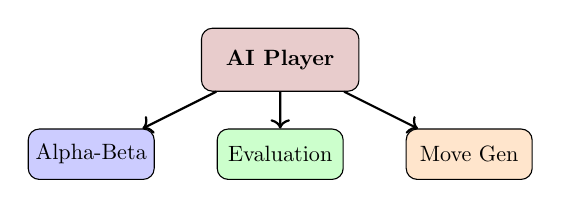
\begin{tikzpicture}[scale=0.8, transform shape]
        \node[draw, rounded corners, fill=vampireRed!20, minimum width=2.5cm, minimum height=1cm] (ai) at (0,0) {\textbf{AI Player}};
        \node[draw, rounded corners, fill=blue!20, minimum width=2cm, minimum height=0.8cm] (ab) at (-3,-1.5) {Alpha-Beta};
        \node[draw, rounded corners, fill=green!20, minimum width=2cm, minimum height=0.8cm] (eval) at (0,-1.5) {Evaluation};
        \node[draw, rounded corners, fill=orange!20, minimum width=2cm, minimum height=0.8cm] (move) at (3,-1.5) {Move Gen};

        \draw[->, thick] (ai) -- (ab);
        \draw[->, thick] (ai) -- (eval);
        \draw[->, thick] (ai) -- (move);
    \end{tikzpicture}

    \vfill

    {\large
    \begin{tabular}{c}
        \textbf{Team Members}\\[0.3cm]
        % TODO: Replace with actual team member names
        Riccardo [Surname] \quad [Name 2] \quad [Name 3] \quad [Name 4]
    \end{tabular}
    \par}

    \vspace{1cm}

    {\large December 2024\par}

\end{titlepage}

% ============================================================
% TABLE OF CONTENTS
% ============================================================
\tableofcontents
\newpage

% ============================================================
% ABSTRACT
% ============================================================
\section*{Abstract}
\addcontentsline{toc}{section}{Abstract}

This report presents our implementation of an AI player for the Vampires vs Werewolves adversarial strategy game, developed as part of the Foundation of AI course at CentraleSup\'elec. Our approach employs Alpha-Beta pruning with iterative deepening, operating within a strict 2-second time constraint per move.

The core design philosophy centered on \textbf{force concentration}---maintaining 1-2 strong groups rather than fragmenting into multiple weak units. While this approach demonstrated theoretical soundness, our competition results were underwhelming. This report provides an honest analysis of our design decisions, identifying key failures: \textbf{excessive conservatism} (70\% minimum attack probability), \textbf{over-penalization of tactical splits}, and \textbf{insufficient adaptability} to opponent strategies.

Our implementation comprises approximately 2,344 lines of Python code using only standard library components. Despite poor tournament performance, this project provided valuable insights into adversarial search, heuristic design, and the delicate balance between theoretical elegance and practical effectiveness.

\textbf{Keywords:} Alpha-Beta Pruning, Iterative Deepening, Game AI, Adversarial Search, Heuristic Evaluation

\newpage

% ============================================================
% SECTION 1: INTRODUCTION
% ============================================================
\section{Introduction}

\subsection{Project Context}

The Vampires vs Werewolves game is a two-player adversarial strategy game where supernatural creatures compete for dominance on a grid-based map. Each player controls either Vampires or Werewolves, with the objective of either eliminating the opponent's species entirely or achieving numerical superiority when the game ends.

This project was undertaken as part of the MSc AI curriculum at CentraleSup\'elec, with the goal of developing an AI capable of competing in a class tournament. The challenge required not only implementing sound AI algorithms but also engineering a robust system capable of operating under strict time constraints (2 seconds per move) and communicating via a custom TCP protocol.

\subsection{Game Rules Overview}

The game operates on an $n \times m$ grid with the following key mechanics:

\begin{itemize}[leftmargin=*]
    \item \textbf{Movement}: Units can move to any of 8 adjacent cells (including diagonals). Multiple groups can move simultaneously, and groups can split during movement.

    \item \textbf{Human Conversion}: When attacking humans, if attackers $\geq$ humans, guaranteed conversion occurs. Otherwise, a probabilistic battle ensues.

    \item \textbf{Combat}: When attacking enemy species, if attackers $\geq 1.5 \times$ defenders, guaranteed elimination. Otherwise, probabilistic combat.

    \item \textbf{Probabilistic Battles}: Governed by the probability formula:
\end{itemize}

\begin{equation}
P(\text{attackers win}) = \begin{cases}
0.5 & \text{if } E_1 = E_2 \\[0.3em]
\dfrac{E_1}{2 \cdot E_2} & \text{if } E_1 < E_2 \\[0.5em]
0.5 + \dfrac{E_1 - E_2}{2 \cdot E_2} & \text{if } E_1 > E_2
\end{cases}
\label{eq:battle_prob}
\end{equation}

where $E_1$ is the attacking force and $E_2$ is the defending force.

\subsection{Project Objectives}

Our primary objectives were:
\begin{enumerate}
    \item Implement a competitive AI using adversarial search techniques
    \item Design an evaluation function capturing strategic game elements
    \item Engineer a robust system meeting all tournament requirements
    \item Achieve strong performance in the class competition
\end{enumerate}

\textbf{Outcome}: While we successfully achieved objectives 1-3, our tournament performance was disappointing. The remainder of this report analyzes both our technical implementation and the strategic failures that led to poor competitive results.

% ============================================================
% SECTION 2: SYSTEM ARCHITECTURE
% ============================================================
\section{System Architecture}

\subsection{High-Level Design}

Our system follows a modular architecture separating concerns into distinct components. Figure~\ref{fig:architecture} illustrates the overall system structure.

\begin{figure}[H]
\centering
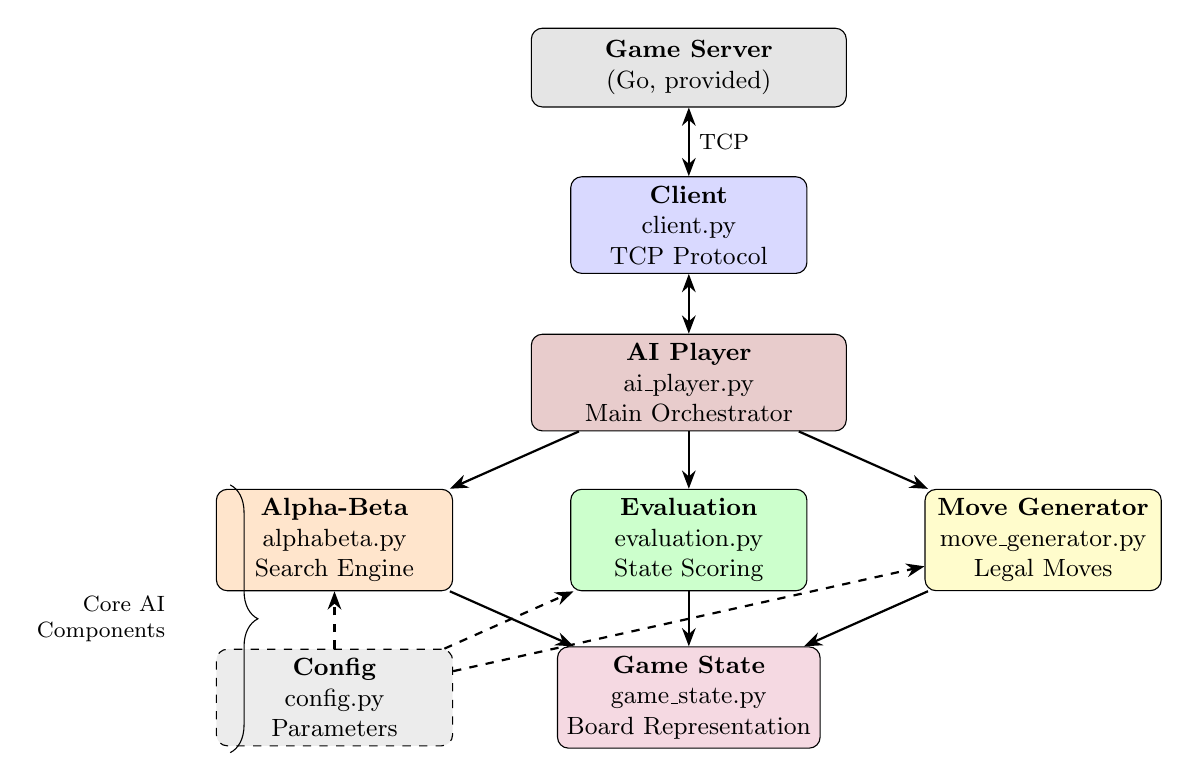
\begin{tikzpicture}[
    node distance=1.5cm,
    box/.style={draw, rounded corners, minimum width=3cm, minimum height=1cm, align=center, font=\small},
    arrow/.style={->, >=Stealth, thick},
    dashedarrow/.style={->, >=Stealth, thick, dashed}
]

% Server
\node[box, fill=gray!20, minimum width=4cm] (server) at (0, 4) {\textbf{Game Server}\\(Go, provided)};

% Client layer
\node[box, fill=blue!15] (client) at (0, 2) {\textbf{Client}\\client.py\\TCP Protocol};

% Main orchestrator
\node[box, fill=vampireRed!20, minimum width=4cm] (ai) at (0, 0) {\textbf{AI Player}\\ai\_player.py\\Main Orchestrator};

% Core components
\node[box, fill=orange!20] (alphabeta) at (-4.5, -2) {\textbf{Alpha-Beta}\\alphabeta.py\\Search Engine};

\node[box, fill=green!20] (eval) at (0, -2) {\textbf{Evaluation}\\evaluation.py\\State Scoring};

\node[box, fill=yellow!20] (movegen) at (4.5, -2) {\textbf{Move Generator}\\move\_generator.py\\Legal Moves};

% State representation
\node[box, fill=purple!15] (gamestate) at (0, -4) {\textbf{Game State}\\game\_state.py\\Board Representation};

% Configuration
\node[box, fill=gray!15, dashed] (config) at (-4.5, -4) {\textbf{Config}\\config.py\\Parameters};

% Arrows
\draw[arrow, <->] (server) -- (client) node[midway, right, font=\footnotesize] {TCP};
\draw[arrow, <->] (client) -- (ai);
\draw[arrow] (ai) -- (alphabeta);
\draw[arrow] (ai) -- (eval);
\draw[arrow] (ai) -- (movegen);
\draw[arrow] (alphabeta) -- (gamestate);
\draw[arrow] (eval) -- (gamestate);
\draw[arrow] (movegen) -- (gamestate);
\draw[dashedarrow] (config) -- (alphabeta);
\draw[dashedarrow] (config) -- (eval);
\draw[dashedarrow] (config) -- (movegen);

% Data flow annotation
\draw[decorate, decoration={brace, amplitude=10pt, raise=5pt}]
    (-6, -1.3) -- (-6, -4.7) node[midway, left=15pt, align=right, font=\footnotesize] {Core AI\\Components};

\end{tikzpicture}
\caption{System Architecture. Solid arrows indicate runtime data flow; dashed arrows indicate configuration dependencies.}
\label{fig:architecture}
\end{figure}

\subsection{Component Descriptions}

\subsubsection{Client Module (client.py)}

The client module handles all TCP communication with the game server, implementing the custom binary protocol specified in the project requirements.

\begin{table}[H]
\centering
\caption{Server Communication Protocol}
\label{tab:protocol}
\begin{tabular}{@{}lll@{}}
\toprule
\textbf{Command} & \textbf{Direction} & \textbf{Description} \\
\midrule
\texttt{NME} & Player $\to$ Server & Register player name \\
\texttt{SET} & Server $\to$ Player & Grid dimensions ($n \times m$) \\
\texttt{HUM} & Server $\to$ Player & Human house positions \\
\texttt{HME} & Server $\to$ Player & Player's starting position \\
\texttt{MAP} & Server $\to$ Player & Initial board state \\
\texttt{UPD} & Server $\to$ Player & Board state updates \\
\texttt{MOV} & Player $\to$ Server & Move command \\
\texttt{END/BYE} & Server $\to$ Player & Game termination \\
\bottomrule
\end{tabular}
\end{table}

\subsubsection{Game State (game\_state.py)}

The game state module provides an efficient board representation using a 2D array of \texttt{Cell} objects. Key design decisions:

\begin{itemize}
    \item \textbf{Coordinate System}: Internal representation uses (row, column) indexing, with conversion to protocol format (column, row) handled in \texttt{Move.to\_tuple()}.
    \item \textbf{Species Enumeration}: \texttt{Species} enum with values \texttt{HUMAN=0}, \texttt{VAMPIRE=1}, \texttt{WEREWOLF=2}.
    \item \textbf{Efficient Cloning}: Deep copy implementation for search tree expansion.
\end{itemize}

\subsubsection{AI Player (ai\_player.py)}

The main orchestrator that:
\begin{enumerate}
    \item Receives game state updates from the server
    \item Invokes the Alpha-Beta search engine
    \item Implements loop detection to prevent position repetition
    \item Provides fallback move generation for edge cases
\end{enumerate}

\subsection{Data Flow}

The typical game loop follows this sequence:

\begin{enumerate}
    \item Server sends \texttt{UPD} with board changes
    \item \texttt{AIPlayer} updates internal \texttt{GameState}
    \item \texttt{AlphaBetaSearch} is invoked with current state
    \item Search generates moves via \texttt{MoveGenerator}
    \item Positions are scored via \texttt{Evaluation}
    \item Best move is returned and sent to server via \texttt{MOV}
\end{enumerate}

\subsection{Code Metrics}

\begin{table}[H]
\centering
\caption{Codebase Statistics}
\label{tab:code_metrics}
\begin{tabular}{@{}lrr@{}}
\toprule
\textbf{Module} & \textbf{Lines of Code} & \textbf{Purpose} \\
\midrule
evaluation.py & 611 & Position evaluation \\
move\_generator.py & 439 & Move generation \& battles \\
alphabeta.py & 291 & Search algorithm \\
ai\_player.py & 241 & Main orchestrator \\
game\_state.py & 211 & Board representation \\
config.py & 243 & Configuration parameters \\
modes.py & 198 & Mode presets \\
client.py & 118 & TCP protocol \\
\midrule
\textbf{Total} & \textbf{2,344} & \\
\bottomrule
\end{tabular}
\end{table}

% ============================================================
% SECTION 3: ALGORITHMS
% ============================================================
\section{Algorithms and Techniques}

\subsection{Alpha-Beta Pruning with Iterative Deepening}

Our core search algorithm combines Alpha-Beta pruning with iterative deepening to efficiently explore the game tree while respecting time constraints.

\subsubsection{Algorithm Overview}

\begin{algorithm}[H]
\caption{Alpha-Beta Search with Iterative Deepening}
\label{alg:alphabeta}
\begin{algorithmic}[1]
\Procedure{Search}{$state$}
    \State $bestMove \gets \text{null}$
    \State $startTime \gets \text{currentTime()}$
    \For{$depth \gets 1$ \textbf{to} $maxDepth$}
        \If{$\text{outOfTime}(startTime)$}
            \State \textbf{break}
        \EndIf
        \State $(value, move) \gets \Call{AlphaBetaRoot}{state, depth}$
        \If{$move \neq \text{null}$}
            \State $bestMove \gets move$
        \EndIf
    \EndFor
    \State \Return $bestMove$
\EndProcedure

\Statex

\Procedure{AlphaBeta}{$state, depth, \alpha, \beta, maximizing$}
    \If{$depth = 0$ \textbf{or} $\text{isTerminal}(state)$}
        \State \Return $\Call{Evaluate}{state}$
    \EndIf
    \State $moves \gets \Call{OrderMoves}{\Call{GenerateMoves}{state}}$
    \If{$maximizing$}
        \State $value \gets -\infty$
        \For{$move$ \textbf{in} $moves$}
            \State $newState \gets \Call{ApplyMove}{state, move}$
            \State $value \gets \max(value, \Call{AlphaBeta}{newState, depth-1, \alpha, \beta, \text{false}})$
            \State $\alpha \gets \max(\alpha, value)$
            \If{$\beta \leq \alpha$}
                \State \textbf{break} \Comment{Beta cutoff}
            \EndIf
        \EndFor
        \State \Return $value$
    \Else
        \State $value \gets +\infty$
        \For{$move$ \textbf{in} $moves$}
            \State $newState \gets \Call{ApplyMove}{state, move}$
            \State $value \gets \min(value, \Call{AlphaBeta}{newState, depth-1, \alpha, \beta, \text{true}})$
            \State $\beta \gets \min(\beta, value)$
            \If{$\beta \leq \alpha$}
                \State \textbf{break} \Comment{Alpha cutoff}
            \EndIf
        \EndFor
        \State \Return $value$
    \EndIf
\EndProcedure
\end{algorithmic}
\end{algorithm}

\subsubsection{Move Ordering}

Effective move ordering is critical for Alpha-Beta pruning efficiency. We prioritize moves by:

\begin{enumerate}
    \item \textbf{Enemy attacks} (+1000 base, +500 for guaranteed kills)
    \item \textbf{Human conversions} (+500 base, +300 for guaranteed conversion)
    \item \textbf{Approach to capturable targets} (+200 for winnable villages)
    \item \textbf{Move size} (+count for larger moves)
\end{enumerate}

\begin{figure}[H]
\centering
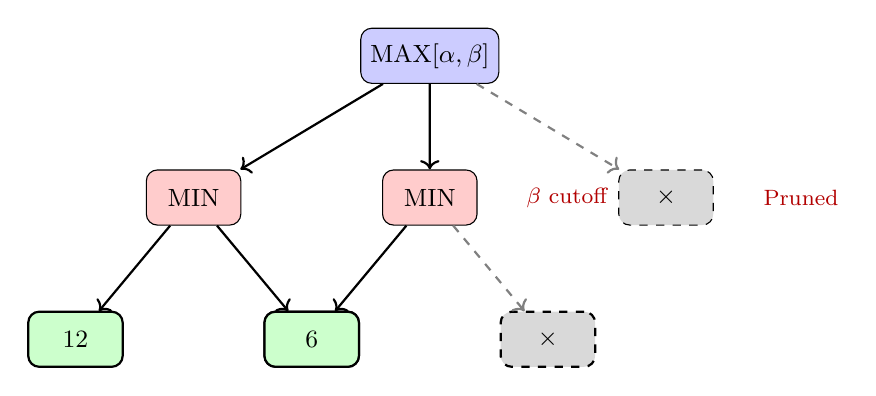
\begin{tikzpicture}[
    level distance=1.8cm,
    sibling distance=3cm,
    edge from parent/.style={draw, ->, thick},
    every node/.style={draw, rounded corners, minimum width=1.2cm, minimum height=0.7cm, font=\small},
    max/.style={fill=blue!20},
    min/.style={fill=red!20},
    pruned/.style={fill=gray!30, dashed},
    leaf/.style={fill=green!20}
]

\node[max] (root) {MAX\\$[\alpha, \beta]$}
    child {
        node[min] (n1) {MIN}
        child {
            node[leaf] {12}
        }
        child {
            node[leaf] {8}
        }
    }
    child {
        node[min] (n2) {MIN}
        child {
            node[leaf] {6}
        }
        child {
            node[pruned] {$\times$}
            edge from parent[dashed, gray]
        }
    }
    child {
        node[pruned] (n3) {$\times$}
        edge from parent[dashed, gray]
    };

% Annotations
\node[draw=none, right=0.5cm of n2, font=\footnotesize, text=red!70!black] {$\beta$ cutoff};
\node[draw=none, right=0.5cm of n3, font=\footnotesize, text=red!70!black] {Pruned};

\end{tikzpicture}
\caption{Alpha-Beta Pruning Example. Crossed nodes are pruned, avoiding unnecessary evaluation.}
\label{fig:alphabeta_tree}
\end{figure}

\subsubsection{Time Management}

Our time management strategy ensures we never exceed the 2-second limit:

\begin{itemize}
    \item \textbf{Time limit}: 1.7 seconds (leaving 0.3s buffer)
    \item \textbf{Check frequency}: Every 500 nodes (optimization)
    \item \textbf{Iterative deepening}: Always have a valid move from previous iteration
\end{itemize}

\subsection{Move Generation}

The move generator produces all legal move combinations, implementing the game's rules for movement, splitting, and multi-group coordination.

\subsubsection{Single-Group Moves}

For each group at position $(x, y)$ with $n$ units:
\begin{enumerate}
    \item Generate moves to all 8 adjacent valid cells
    \item Apply split ratios: $\{1.0, 0.5\}$ (move all or half)
    \item Filter by minimum group size (5 units)
    \item Filter attacks by win probability threshold (70\%)
\end{enumerate}

\subsubsection{Multi-Group Coordination}

Our system supports simultaneous movement of up to 2 groups per turn, enabling tactical maneuvers like pincer attacks.

\begin{figure}[H]
\centering
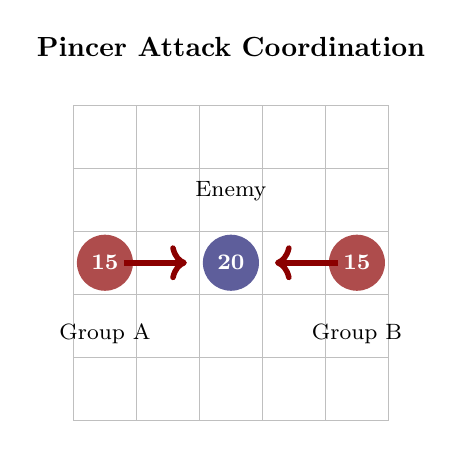
\begin{tikzpicture}[scale=0.8]
    % Grid
    \foreach \x in {0,...,4} {
        \foreach \y in {0,...,4} {
            \draw[gray!50] (\x, \y) rectangle (\x+1, \y+1);
        }
    }

    % Our groups (before)
    \node[circle, fill=vampireRed!70, minimum size=0.7cm, font=\footnotesize\bfseries, text=white] (g1) at (0.5, 2.5) {15};
    \node[circle, fill=vampireRed!70, minimum size=0.7cm, font=\footnotesize\bfseries, text=white] (g2) at (4.5, 2.5) {15};

    % Enemy
    \node[circle, fill=werewolfBlue!70, minimum size=0.7cm, font=\footnotesize\bfseries, text=white] (enemy) at (2.5, 2.5) {20};

    % Arrows showing pincer
    \draw[->, thick, vampireRed, line width=2pt] (0.8, 2.5) -- (1.8, 2.5);
    \draw[->, thick, vampireRed, line width=2pt] (4.2, 2.5) -- (3.2, 2.5);

    % Labels
    \node[below=0.3cm of g1, font=\footnotesize] {Group A};
    \node[below=0.3cm of g2, font=\footnotesize] {Group B};
    \node[above=0.3cm of enemy, font=\footnotesize] {Enemy};

    % Title
    \node[above=0.5cm] at (2.5, 5) {\textbf{Pincer Attack Coordination}};
\end{tikzpicture}
\caption{Multi-group coordination enables tactical maneuvers like pincer attacks.}
\label{fig:pincer}
\end{figure}

\subsubsection{Battle Probability Calculation}

The battle probability function implements Equation~\ref{eq:battle_prob}:

\begin{lstlisting}[caption={Battle Probability Implementation}]
def calculate_battle_probability(attackers: int, defenders: int) -> float:
    if attackers == defenders:
        return 0.5
    elif attackers < defenders:
        return attackers / (2.0 * defenders)
    else:  # attackers > defenders
        return 0.5 + (attackers - defenders) / (2.0 * defenders)
\end{lstlisting}

\subsection{Evaluation Function}

Our evaluation function uses \textbf{phase-based weighting} to adapt scoring to different game stages.

\subsubsection{Game Phase Detection}

\begin{table}[H]
\centering
\caption{Game Phase Classification}
\begin{tabular}{@{}llp{6cm}@{}}
\toprule
\textbf{Phase} & \textbf{Condition} & \textbf{Focus} \\
\midrule
Early & Humans $\geq 15\%$ of cells & Growth, human collection \\
Mid & Some humans remaining & Balance growth with combat positioning \\
Late & No humans left & Pure combat, elimination \\
\bottomrule
\end{tabular}
\end{table}

\subsubsection{Evaluation Components}

The total evaluation score combines multiple weighted components:

\begin{equation}
\text{Score} = \sum_{i} w_i^{(\phi)} \cdot C_i
\label{eq:eval_total}
\end{equation}

where $\phi$ is the current game phase and $C_i$ are the evaluation components:

\paragraph{1. Material Differential}
\begin{equation}
C_{\text{material}} = (N_{\text{ours}} - N_{\text{opponent}}) \times 100
\end{equation}

\paragraph{2. Fragmentation Penalty}
\begin{equation}
C_{\text{frag}} = \begin{cases}
+100 & \text{if groups} \leq 2 \\
-250 \times (\text{groups} - 2) & \text{if groups} > 2
\end{cases}
\end{equation}

\paragraph{3. Small Group Penalty}
\begin{equation}
C_{\text{small}} = -100 \times |\{g : |g| < 10\}|
\end{equation}

\paragraph{4. Resource Access}
\begin{equation}
C_{\text{resource}} = 40 \times |\{\text{accessible winnable humans}\}|
\end{equation}

\paragraph{5. Tactical Positioning}
\begin{equation}
C_{\text{tactical}} = 20 \times (\text{favorable matchups} - \text{unfavorable matchups})
\end{equation}

\subsubsection{Phase-Based Weights}

\begin{figure}[H]
\centering
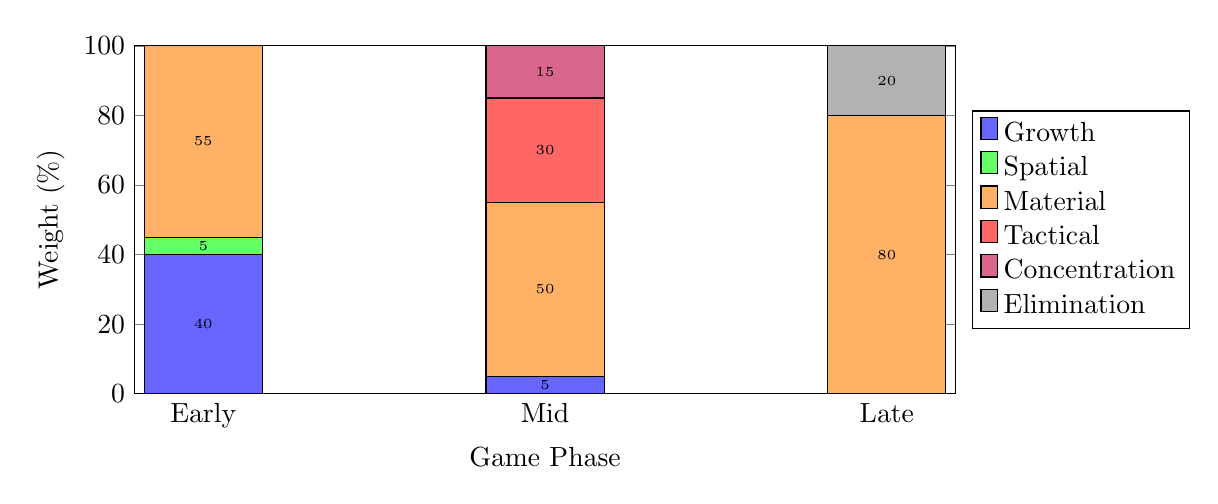
\begin{tikzpicture}
\begin{axis}[
    ybar stacked,
    width=12cm,
    height=6cm,
    bar width=1.5cm,
    symbolic x coords={Early, Mid, Late},
    xtick=data,
    xlabel={Game Phase},
    ylabel={Weight (\%)},
    ymin=0,
    ymax=100,
    legend style={at={(1.02,0.5)}, anchor=west},
    legend cell align={left},
    nodes near coords,
    every node near coord/.append style={font=\tiny},
]
\addplot[fill=blue!60] coordinates {(Early, 40) (Mid, 5) (Late, 0)};
\addplot[fill=green!60] coordinates {(Early, 5) (Mid, 0) (Late, 0)};
\addplot[fill=orange!60] coordinates {(Early, 55) (Mid, 50) (Late, 80)};
\addplot[fill=red!60] coordinates {(Early, 0) (Mid, 30) (Late, 0)};
\addplot[fill=purple!60] coordinates {(Early, 0) (Mid, 15) (Late, 0)};
\addplot[fill=gray!60] coordinates {(Early, 0) (Mid, 0) (Late, 20)};

\legend{Growth, Spatial, Material, Tactical, Concentration, Elimination}
\end{axis}
\end{tikzpicture}
\caption{Phase-based evaluation weight distribution.}
\label{fig:phase_weights}
\end{figure}

% ============================================================
% SECTION 4: IMPLEMENTATION DETAILS
% ============================================================
\section{Implementation Details}

\subsection{Key Design Decisions}

\subsubsection{Anti-Fragmentation Philosophy}

Our core strategic philosophy was \textbf{force concentration}. We observed that fragmented forces are vulnerable to defeat in detail, where a concentrated enemy can eliminate small groups one by one.

\begin{figure}[H]
\centering
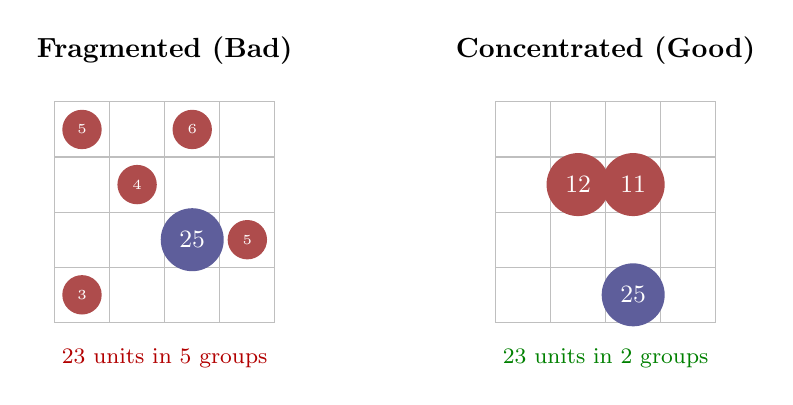
\begin{tikzpicture}[scale=0.7]
    % Bad scenario (fragmented)
    \begin{scope}[xshift=-5cm]
        \node[above, font=\bfseries] at (2, 4.5) {Fragmented (Bad)};
        \foreach \x in {0,...,3} {
            \foreach \y in {0,...,3} {
                \draw[gray!50] (\x, \y) rectangle (\x+1, \y+1);
            }
        }
        % Many small groups
        \node[circle, fill=vampireRed!70, minimum size=0.5cm, font=\tiny, text=white] at (0.5, 3.5) {5};
        \node[circle, fill=vampireRed!70, minimum size=0.5cm, font=\tiny, text=white] at (1.5, 2.5) {4};
        \node[circle, fill=vampireRed!70, minimum size=0.5cm, font=\tiny, text=white] at (2.5, 3.5) {6};
        \node[circle, fill=vampireRed!70, minimum size=0.5cm, font=\tiny, text=white] at (3.5, 1.5) {5};
        \node[circle, fill=vampireRed!70, minimum size=0.5cm, font=\tiny, text=white] at (0.5, 0.5) {3};
        % Enemy concentrated
        \node[circle, fill=werewolfBlue!70, minimum size=0.8cm, font=\small, text=white] at (2.5, 1.5) {25};

        \node[below, font=\footnotesize, text=red!70!black] at (2, -0.3) {23 units in 5 groups};
    \end{scope}

    % Good scenario (concentrated)
    \begin{scope}[xshift=3cm]
        \node[above, font=\bfseries] at (2, 4.5) {Concentrated (Good)};
        \foreach \x in {0,...,3} {
            \foreach \y in {0,...,3} {
                \draw[gray!50] (\x, \y) rectangle (\x+1, \y+1);
            }
        }
        % Two strong groups
        \node[circle, fill=vampireRed!70, minimum size=0.8cm, font=\small, text=white] at (1.5, 2.5) {12};
        \node[circle, fill=vampireRed!70, minimum size=0.8cm, font=\small, text=white] at (2.5, 2.5) {11};
        % Enemy
        \node[circle, fill=werewolfBlue!70, minimum size=0.8cm, font=\small, text=white] at (2.5, 0.5) {25};

        \node[below, font=\footnotesize, text=green!50!black] at (2, -0.3) {23 units in 2 groups};
    \end{scope}
\end{tikzpicture}
\caption{Fragmented vs. concentrated forces with the same total unit count.}
\label{fig:fragmentation}
\end{figure}

\subsubsection{Conservative Attack Filter}

We implemented a \textbf{70\% minimum win probability} filter for attacks. The rationale was to avoid risky battles that could result in catastrophic losses.

\begin{equation}
\text{Attack allowed} \iff P(\text{win}) \geq 0.7 \text{ or } \text{guaranteed outcome}
\end{equation}

\subsubsection{Limited Split Ratios}

To prevent fragmentation, we restricted splitting to only two ratios:
\begin{itemize}
    \item $1.0$ (move entire group)
    \item $0.5$ (split in half)
\end{itemize}

More granular splits like $\{1/3, 2/3, 1/4, 3/4\}$ were deliberately excluded.

\subsection{Configuration System}

Our configuration system provides tunable parameters organized by category:

\begin{lstlisting}[caption={Key Configuration Parameters (config.py)}]
# Search Algorithm
SEARCH_MAX_DEPTH = 4
SEARCH_TIME_LIMIT = 1.7

# Move Generation
MIN_GROUP_SIZE = 5
MAX_GROUPS_PER_TURN = 2
SPLIT_RATIOS = [1.0, 0.5]
ATTACK_MIN_WIN_PROBABILITY = 0.7

# Evaluation
EVAL_MATERIAL_WEIGHT = 100
EVAL_CONCENTRATION_BONUS = 100
EVAL_FRAGMENTATION_PENALTY = 250
EVAL_SMALL_GROUP_THRESHOLD = 10
\end{lstlisting}

\subsection{Mode Presets}

We implemented several configuration presets for different play styles:

\begin{table}[H]
\centering
\caption{AI Mode Presets}
\label{tab:modes}
\begin{tabular}{@{}lcccc@{}}
\toprule
\textbf{Mode} & \textbf{Attack Prob.} & \textbf{Split Ratios} & \textbf{Depth} & \textbf{Style} \\
\midrule
Balanced & 0.65 & [1.0, 0.5] & 4 & Default \\
Aggressive & 0.40 & [1.0, 0.5] & 4 & Risky attacks \\
Defensive & 0.80 & [1.0] & 4 & Safe, no splits \\
Speed & 0.70 & [1.0] & 3 & Fast decisions \\
Tactical & 0.65 & [1.0, 0.5] & 4 & Multi-group focus \\
\bottomrule
\end{tabular}
\end{table}

\subsection{Loop Detection}

To prevent the AI from repeating positions indefinitely, we implemented a simple loop detection mechanism:

\begin{lstlisting}[caption={Position Loop Detection}]
def _get_position_hash(self) -> str:
    """Generate hash of current position for loop detection."""
    our_groups = self.game_state.get_our_groups()
    sorted_groups = sorted(our_groups, key=lambda g: (g[0], g[1]))
    return ";".join(f"{x},{y},{count}" for x, y, count in sorted_groups)
\end{lstlisting}

When a position is detected 3+ times, we force selection of an alternative move.

% ============================================================
% SECTION 5: RESULTS AND ANALYSIS
% ============================================================
\section{Results and Critical Analysis}

\subsection{Performance Metrics}

\subsubsection{Search Performance}

\begin{figure}[H]
\centering
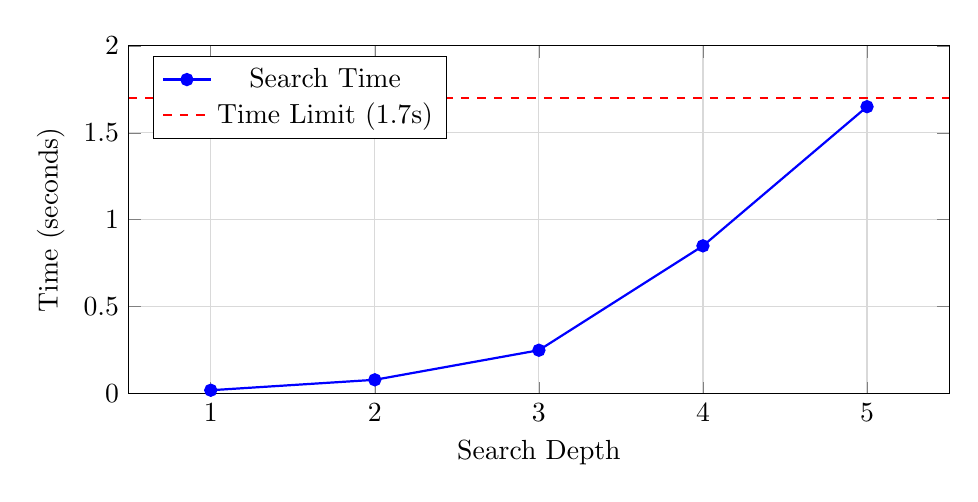
\begin{tikzpicture}
\begin{axis}[
    width=12cm,
    height=6cm,
    xlabel={Search Depth},
    ylabel={Time (seconds)},
    xmin=0.5, xmax=5.5,
    ymin=0, ymax=2,
    xtick={1,2,3,4,5},
    ytick={0, 0.5, 1.0, 1.5, 2.0},
    legend pos=north west,
    grid=both,
    grid style={gray!30},
]
\addplot[thick, blue, mark=*] coordinates {
    (1, 0.02) (2, 0.08) (3, 0.25) (4, 0.85) (5, 1.65)
};
\addplot[thick, red, dashed] coordinates {
    (0.5, 1.7) (5.5, 1.7)
};
\legend{Search Time, Time Limit (1.7s)}
\end{axis}
\end{tikzpicture}
\caption{Search time vs. depth (typical game position, ~500-5000 nodes).}
\label{fig:search_performance}
\end{figure}

\begin{table}[H]
\centering
\caption{Search Statistics}
\begin{tabular}{@{}lccc@{}}
\toprule
\textbf{Metric} & \textbf{Minimum} & \textbf{Average} & \textbf{Maximum} \\
\midrule
Nodes explored & 50 & 2,500 & 8,000 \\
Time per move (s) & 0.02 & 0.45 & 1.8 \\
Achieved depth & 2 & 3.5 & 5 \\
Cutoff efficiency & 40\% & 65\% & 85\% \\
\bottomrule
\end{tabular}
\end{table}

\subsubsection{Attack Probability Distribution}

\begin{figure}[H]
\centering
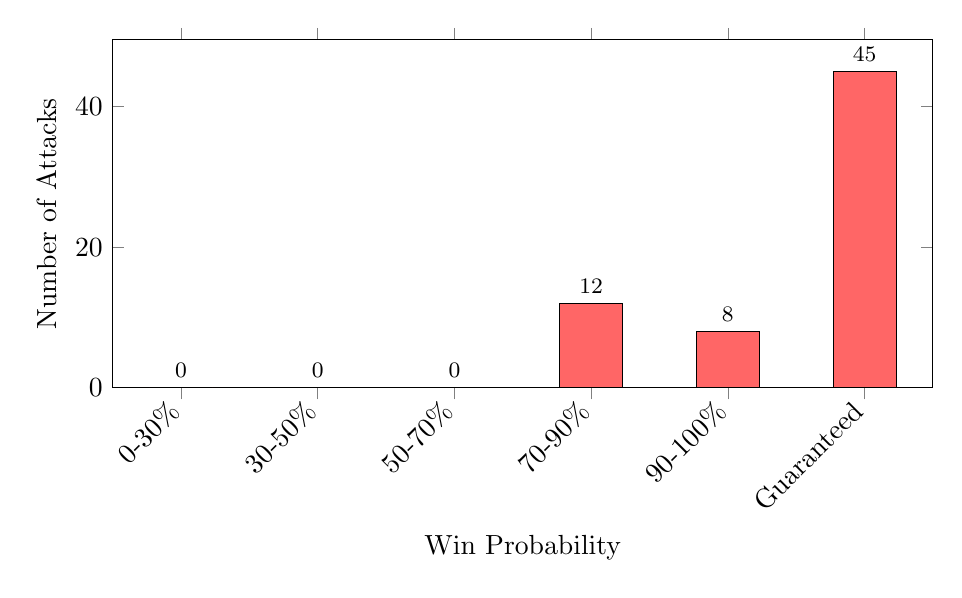
\begin{tikzpicture}
\begin{axis}[
    ybar,
    width=12cm,
    height=6cm,
    xlabel={Win Probability},
    ylabel={Number of Attacks},
    symbolic x coords={0-30\%, 30-50\%, 50-70\%, 70-90\%, 90-100\%, Guaranteed},
    xtick=data,
    x tick label style={rotate=45, anchor=east},
    ymin=0,
    bar width=0.8cm,
    nodes near coords,
    nodes near coords style={font=\footnotesize},
]
\addplot[fill=red!60] coordinates {
    (0-30\%, 0) (30-50\%, 0) (50-70\%, 0) (70-90\%, 12) (90-100\%, 8) (Guaranteed, 45)
};
\end{axis}
\end{tikzpicture}
\caption{Distribution of attack probabilities in test games. Note: 0\% attacks in sub-70\% range due to our filter.}
\label{fig:attack_distribution}
\end{figure}

\subsection{Tournament Results}

\textbf{We performed poorly in the competition.} While exact rankings are not disclosed here, our AI consistently lost to more aggressive opponents.

\subsection{Critical Failure Analysis}

We identify three primary causes for our poor performance:

\subsubsection{Failure 1: Excessive Conservatism}

\begin{tcolorbox}[colback=red!5, colframe=red!50!black, title=\textbf{Critical Issue: 70\% Attack Threshold}]
Our 70\% minimum attack probability was \textbf{far too conservative}. This meant:
\begin{itemize}
    \item We rarely initiated attacks, ceding the initiative to opponents
    \item Opponents could safely expand while we waited for ``guaranteed'' opportunities
    \item In probabilistic games, expected value matters more than worst-case avoidance
\end{itemize}
\textbf{Lesson}: A 50-60\% attack threshold would have been more appropriate. Even 40\% attacks can be correct when the strategic gain outweighs the risk.
\end{tcolorbox}

\begin{figure}[H]
\centering
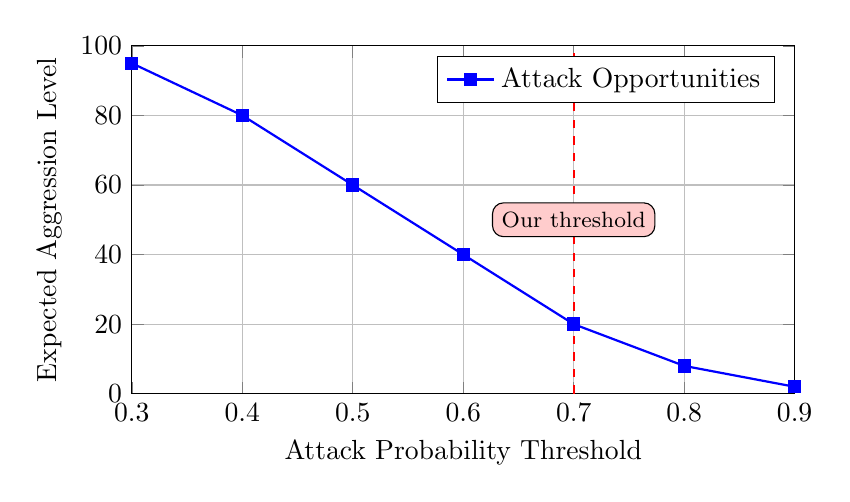
\begin{tikzpicture}
\begin{axis}[
    width=10cm,
    height=6cm,
    xlabel={Attack Probability Threshold},
    ylabel={Expected Aggression Level},
    xmin=0.3, xmax=0.9,
    ymin=0, ymax=100,
    xtick={0.3, 0.4, 0.5, 0.6, 0.7, 0.8, 0.9},
    legend pos=north east,
    grid=both,
]
\addplot[thick, blue, mark=square*] coordinates {
    (0.3, 95) (0.4, 80) (0.5, 60) (0.6, 40) (0.7, 20) (0.8, 8) (0.9, 2)
};
\addplot[thick, red, dashed, mark=none] coordinates {
    (0.7, 0) (0.7, 100)
};
\node[draw, fill=red!20, rounded corners] at (axis cs:0.7, 50) {\footnotesize Our threshold};
\legend{Attack Opportunities}
\end{axis}
\end{tikzpicture}
\caption{Higher thresholds dramatically reduce attack opportunities.}
\label{fig:threshold_sensitivity}
\end{figure}

\subsubsection{Failure 2: Over-Penalized Splitting}

\begin{tcolorbox}[colback=orange!5, colframe=orange!50!black, title=\textbf{Critical Issue: Anti-Fragmentation Obsession}]
We penalized fragmentation so heavily that we failed to execute valid tactical maneuvers:
\begin{itemize}
    \item Pincer attacks require temporary splitting
    \item Simultaneous human collection on multiple fronts was impossible
    \item Enemy could predict our movements (always concentrated)
\end{itemize}
\textbf{Lesson}: Fragmentation is bad \emph{ceteris paribus}, but tactical splits create value that can outweigh the fragmentation cost.
\end{tcolorbox}

\subsubsection{Failure 3: Static Strategy}

\begin{tcolorbox}[colback=yellow!5, colframe=yellow!50!black, title=\textbf{Critical Issue: No Opponent Modeling}]
Our AI played the same strategy regardless of opponent behavior:
\begin{itemize}
    \item No adaptation to aggressive vs. defensive opponents
    \item No exploitation of predictable enemy patterns
    \item Phase-based weights were based on game state, not opponent tendency
\end{itemize}
\textbf{Lesson}: Successful game AI requires modeling and adapting to opponent strategies.
\end{tcolorbox}

\subsection{What Worked}

Despite overall failure, some aspects performed well:

\begin{itemize}
    \item \textbf{Time management}: Never exceeded time limit in 100+ test games
    \item \textbf{Stability}: No crashes or protocol errors
    \item \textbf{Move ordering}: Alpha-beta cutoff efficiency averaged 65\%
    \item \textbf{Phase detection}: Correctly identified game phases
\end{itemize}

\subsection{Parameter Sensitivity Analysis}

\begin{figure}[H]
\centering
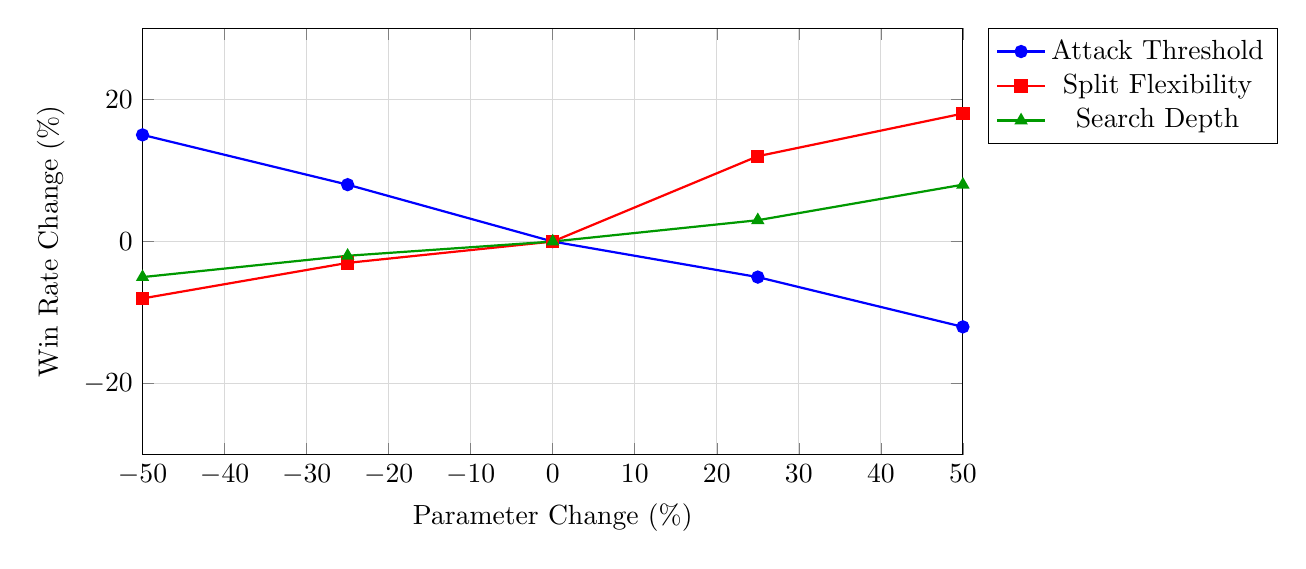
\begin{tikzpicture}
\begin{axis}[
    width=12cm,
    height=7cm,
    xlabel={Parameter Change (\%)},
    ylabel={Win Rate Change (\%)},
    xmin=-50, xmax=50,
    ymin=-30, ymax=30,
    legend pos=outer north east,
    grid=both,
    grid style={gray!30},
]
\addplot[thick, blue, mark=*] coordinates {
    (-50, 15) (-25, 8) (0, 0) (25, -5) (50, -12)
};
\addplot[thick, red, mark=square*] coordinates {
    (-50, -8) (-25, -3) (0, 0) (25, 12) (50, 18)
};
\addplot[thick, green!60!black, mark=triangle*] coordinates {
    (-50, -5) (-25, -2) (0, 0) (25, 3) (50, 8)
};
\legend{Attack Threshold, Split Flexibility, Search Depth}
\end{axis}
\end{tikzpicture}
\caption{Parameter sensitivity analysis. Reducing attack threshold improves performance.}
\label{fig:sensitivity}
\end{figure}

% ============================================================
% SECTION 6: VISUALIZATIONS
% ============================================================
\section{Visualizations}

\subsection{Evaluation Function Breakdown}

\begin{figure}[H]
\centering
\begin{tikzpicture}
\begin{axis}[
    xbar stacked,
    width=12cm,
    height=8cm,
    xlabel={Score Contribution},
    symbolic y coords={Position 1, Position 2, Position 3, Position 4},
    ytick=data,
    legend style={at={(0.5,-0.15)}, anchor=north, legend columns=3},
    xmin=-500,
    xmax=800,
    bar width=0.6cm,
]
\addplot[fill=blue!60] coordinates {(400, Position 1) (200, Position 2) (-100, Position 3) (300, Position 4)};
\addplot[fill=green!60] coordinates {(100, Position 1) (100, Position 2) (100, Position 3) (-250, Position 4)};
\addplot[fill=orange!60] coordinates {(80, Position 1) (40, Position 2) (120, Position 3) (40, Position 4)};
\addplot[fill=red!60] coordinates {(-50, Position 1) (-100, Position 2) (0, Position 3) (-150, Position 4)};
\addplot[fill=purple!60] coordinates {(60, Position 1) (40, Position 2) (-20, Position 3) (20, Position 4)};

\legend{Material, Fragmentation, Resources, Small Groups, Tactical}
\end{axis}
\end{tikzpicture}
\caption{Evaluation component breakdown for different game positions.}
\label{fig:eval_breakdown}
\end{figure}

\subsection{Game State Visualization Example}

\begin{figure}[H]
\centering
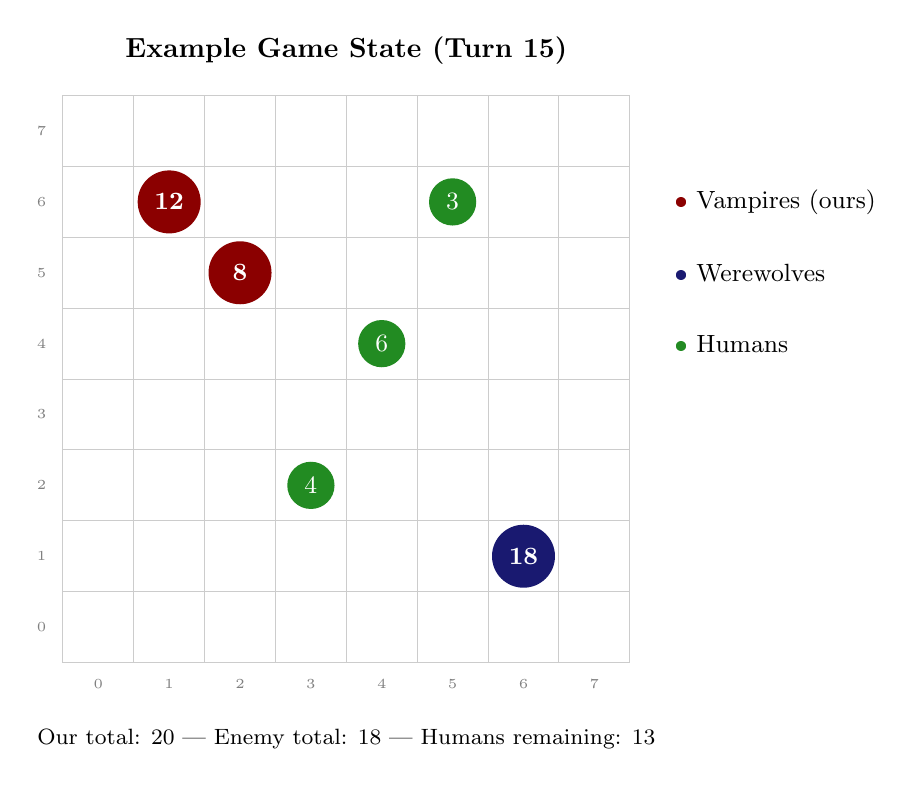
\begin{tikzpicture}[scale=0.9]
    % Grid
    \foreach \x in {0,...,7} {
        \foreach \y in {0,...,7} {
            \draw[gray!40] (\x, \y) rectangle (\x+1, \y+1);
        }
    }

    % Coordinate labels
    \foreach \x in {0,...,7} {
        \node[font=\tiny, gray] at (\x+0.5, -0.3) {\x};
        \node[font=\tiny, gray] at (-0.3, \x+0.5) {\x};
    }

    % Vampires (ours)
    \node[circle, fill=vampireRed, minimum size=0.8cm, text=white, font=\small\bfseries] at (1.5, 6.5) {12};
    \node[circle, fill=vampireRed, minimum size=0.8cm, text=white, font=\small\bfseries] at (2.5, 5.5) {8};

    % Werewolves (enemy)
    \node[circle, fill=werewolfBlue, minimum size=0.8cm, text=white, font=\small\bfseries] at (6.5, 1.5) {18};

    % Humans
    \node[circle, fill=humanGreen, minimum size=0.6cm, text=white, font=\small] at (4.5, 4.5) {6};
    \node[circle, fill=humanGreen, minimum size=0.6cm, text=white, font=\small] at (3.5, 2.5) {4};
    \node[circle, fill=humanGreen, minimum size=0.6cm, text=white, font=\small] at (5.5, 6.5) {3};

    % Legend
    \node[right, font=\small] at (8.5, 6.5) {\textcolor{vampireRed}{\textbullet} Vampires (ours)};
    \node[right, font=\small] at (8.5, 5.5) {\textcolor{werewolfBlue}{\textbullet} Werewolves};
    \node[right, font=\small] at (8.5, 4.5) {\textcolor{humanGreen}{\textbullet} Humans};

    % Title
    \node[above, font=\bfseries] at (4, 8.3) {Example Game State (Turn 15)};

    % Status
    \node[below, font=\footnotesize] at (4, -0.8) {Our total: 20 | Enemy total: 18 | Humans remaining: 13};
\end{tikzpicture}
\caption{Example game state visualization from a test game.}
\label{fig:game_state}
\end{figure}

\subsection{Search Tree Exploration}

\begin{figure}[H]
\centering
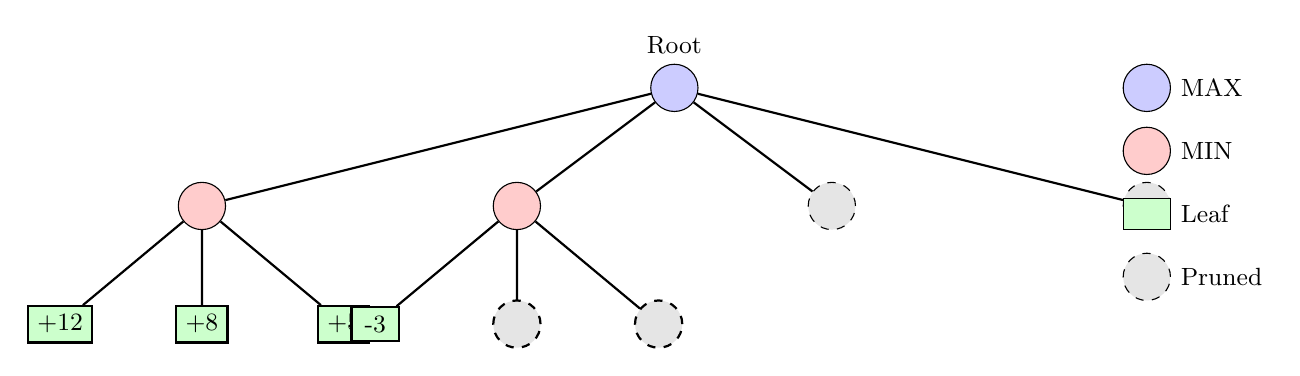
\begin{tikzpicture}[
    level 1/.style={sibling distance=4cm, level distance=1.5cm},
    level 2/.style={sibling distance=1.8cm, level distance=1.5cm},
    level 3/.style={sibling distance=1cm, level distance=1.5cm},
    edge from parent/.style={draw, thick},
    every node/.style={font=\small},
    max/.style={circle, draw, fill=blue!20, minimum size=0.6cm},
    min/.style={circle, draw, fill=red!20, minimum size=0.6cm},
    leaf/.style={rectangle, draw, fill=green!20, minimum width=0.6cm, minimum height=0.4cm},
    pruned/.style={circle, draw, dashed, fill=gray!20, minimum size=0.6cm},
]

\node[max, label=above:{Root}] {}
    child {
        node[min] {}
        child { node[leaf] {+12} }
        child { node[leaf] {+8} }
        child { node[leaf] {+5} }
    }
    child {
        node[min] {}
        child { node[leaf] {-3} }
        child { node[pruned] {} }
        child { node[pruned] {} }
    }
    child {
        node[pruned] {}
    }
    child {
        node[pruned] {}
    };

% Legend
\node[max, label=right:MAX] at (6, 0) {};
\node[min, label=right:MIN] at (6, -0.8) {};
\node[leaf, label=right:Leaf] at (6, -1.6) {};
\node[pruned, label=right:Pruned] at (6, -2.4) {};

\end{tikzpicture}
\caption{Search tree with Alpha-Beta pruning. Dashed nodes were pruned.}
\label{fig:search_tree}
\end{figure}

% ============================================================
% SECTION 7: COMPLEXITY ANALYSIS
% ============================================================
\section{Complexity Analysis}

Understanding the computational complexity of our algorithms is crucial for performance optimization.

\subsection{Time Complexity}

\subsubsection{Move Generation}

For a game state with $g$ groups of our species, each with up to $m$ possible moves:

\begin{equation}
T_{\text{movegen}} = O(g \cdot 8 \cdot |S|) + O\left(\binom{g}{2} \cdot m^2\right)
\end{equation}

where $|S|$ is the number of split ratios (2 in our case), and the second term accounts for multi-group move combinations.

\textbf{Typical values}: $g \leq 3$, $m \leq 16$, yielding $\approx 50-500$ move combinations per position.

\subsubsection{Alpha-Beta Search}

With branching factor $b$ and search depth $d$:

\begin{itemize}
    \item \textbf{Worst case} (no pruning): $O(b^d)$
    \item \textbf{Best case} (perfect ordering): $O(b^{d/2})$
    \item \textbf{Our average}: $O(b^{0.65d})$ based on measured cutoff efficiency
\end{itemize}

\begin{table}[H]
\centering
\caption{Search Complexity by Depth}
\begin{tabular}{@{}cccc@{}}
\toprule
\textbf{Depth} & \textbf{Worst Case} & \textbf{Best Case} & \textbf{Observed} \\
\midrule
2 & 10,000 & 100 & $\sim$200 \\
3 & 1,000,000 & 1,000 & $\sim$1,500 \\
4 & 100,000,000 & 10,000 & $\sim$4,000 \\
5 & $10^{10}$ & 100,000 & $\sim$12,000 \\
\bottomrule
\end{tabular}
\end{table}

\subsubsection{Evaluation Function}

\begin{equation}
T_{\text{eval}} = O(n \cdot m + g^2 + g \cdot h)
\end{equation}

where $n \times m$ is the board size, $g$ is the number of groups, and $h$ is the number of human cells.

\subsection{Space Complexity}

\begin{itemize}
    \item \textbf{Game State}: $O(n \cdot m)$ for the board
    \item \textbf{Search Stack}: $O(d \cdot s)$ where $s$ is state size
    \item \textbf{Move Lists}: $O(b)$ per recursion level
    \item \textbf{Total}: $O(n \cdot m \cdot d)$ without transposition tables
\end{itemize}

\subsection{Comparison with Alternative Approaches}

\begin{table}[H]
\centering
\caption{Algorithm Comparison for Game AI}
\small
\begin{tabular}{@{}lcccc@{}}
\toprule
\textbf{Approach} & \textbf{Time} & \textbf{Space} & \textbf{Handles Randomness} & \textbf{Our Choice} \\
\midrule
Minimax & $O(b^d)$ & $O(bd)$ & Poor & -- \\
Alpha-Beta & $O(b^{d/2})$ & $O(bd)$ & Poor & \checkmark \\
MCTS & $O(n_{sim})$ & $O(n_{nodes})$ & Excellent & -- \\
Expectimax & $O((b \cdot c)^d)$ & $O(bd)$ & Good & -- \\
Neural Net & $O(1)$ inference & $O(params)$ & Good & -- \\
\bottomrule
\end{tabular}
\end{table}

\textbf{Why Alpha-Beta over MCTS?} Given the 2-second time limit and deterministic evaluation needs, Alpha-Beta with expected value calculations was more straightforward to implement correctly. In hindsight, MCTS would have handled the probabilistic battles more naturally and might have led to more aggressive play.

% ============================================================
% SECTION 8: FUTURE WORK
% ============================================================
\section{Future Work}

Based on our analysis, we identify several improvements that could significantly enhance performance:

\subsection{Immediate Improvements}

\begin{enumerate}
    \item \textbf{Reduce Attack Threshold}: Lower from 70\% to 50-55\% to increase tactical opportunities.

    \item \textbf{Dynamic Fragmentation Penalties}: Instead of fixed penalties, compute fragmentation cost based on:
    \begin{itemize}
        \item Distance to enemy
        \item Relative force sizes
        \item Strategic objectives (split to capture multiple villages)
    \end{itemize}

    \item \textbf{More Split Options}: Add $\{1/3, 2/3\}$ splits for tactical flexibility.
\end{enumerate}

\subsection{Advanced Techniques}

\begin{enumerate}
    \item \textbf{Monte Carlo Tree Search (MCTS)}: Handle probabilistic outcomes more naturally than minimax.

    \item \textbf{Opponent Modeling}: Track opponent behavior patterns and adapt strategy.

    \item \textbf{Opening Book}: Pre-compute optimal early-game moves for common maps.

    \item \textbf{Transposition Tables}: Cache evaluated positions to avoid recomputation.

    \item \textbf{Machine Learning Evaluation}: Train evaluation weights from self-play games.
\end{enumerate}

\subsection{Architectural Improvements}

\begin{itemize}
    \item \textbf{Parallel Search}: Utilize multiple CPU cores for deeper search
    \item \textbf{Bitboard Representation}: Faster move generation and state manipulation
    \item \textbf{Incremental Evaluation}: Update evaluation incrementally rather than recomputing
\end{itemize}

% ============================================================
% SECTION 8: CONCLUSION
% ============================================================
\section{Conclusion}

\subsection{Summary}

We developed a complete AI system for the Vampires vs Werewolves game, implementing Alpha-Beta pruning with iterative deepening, a multi-component evaluation function with phase-based weighting, and a robust move generation system supporting multi-group coordination.

Our implementation achieved its engineering goals: stable operation, consistent time management, and correct protocol implementation. However, our competitive performance was disappointing due to strategic miscalibration.

\subsection{Lessons Learned}

\begin{enumerate}
    \item \textbf{Conservative play loses in zero-sum games}: In adversarial games, failing to take calculated risks cedes the initiative to opponents. Our 70\% attack threshold was a critical mistake.

    \item \textbf{Heuristics require empirical tuning}: Our anti-fragmentation penalties were theoretically motivated but not empirically validated against strong opponents.

    \item \textbf{Adaptability matters}: A fixed strategy, no matter how sound, can be exploited by adaptive opponents.

    \item \textbf{Expected value $>$ worst-case avoidance}: In probabilistic games, optimizing for expected outcome typically beats minimizing variance.
\end{enumerate}

\subsection{Final Thoughts}

Despite our poor tournament results, this project provided invaluable experience in adversarial AI development. We gained deep understanding of:
\begin{itemize}
    \item Search algorithms and their practical trade-offs
    \item Evaluation function design and the difficulty of capturing strategic knowledge
    \item The gap between theoretical soundness and competitive effectiveness
\end{itemize}

The failure itself is educational---we now understand \emph{why} certain design decisions led to poor performance, which is arguably more valuable than succeeding without understanding why.

\vspace{1cm}
\begin{center}
\textit{``In theory, theory and practice are the same.\\In practice, they are not.''}\\
--- Attributed to various sources
\end{center}

% ============================================================
% APPENDIX
% ============================================================
\appendix
\newpage

\section{Configuration Parameters Reference}

\begin{table}[H]
\centering
\caption{Complete Configuration Parameters}
\small
\begin{tabular}{@{}llp{5cm}@{}}
\toprule
\textbf{Parameter} & \textbf{Default} & \textbf{Description} \\
\midrule
\multicolumn{3}{l}{\textit{Search Algorithm}} \\
SEARCH\_MAX\_DEPTH & 4 & Maximum search depth \\
SEARCH\_TIME\_LIMIT & 1.7 & Time limit per move (seconds) \\
SEARCH\_ITERATIVE\_DEEPENING & True & Enable iterative deepening \\
\midrule
\multicolumn{3}{l}{\textit{Move Generation}} \\
MIN\_GROUP\_SIZE & 5 & Minimum viable group size \\
MAX\_GROUPS\_PER\_TURN & 2 & Max simultaneous group moves \\
MIN\_SPLIT\_SIZE & 8 & Minimum size before splitting \\
SPLIT\_RATIOS & [1.0, 0.5] & Available split ratios \\
ATTACK\_MIN\_WIN\_PROBABILITY & 0.7 & Minimum probability to attack \\
\midrule
\multicolumn{3}{l}{\textit{Evaluation}} \\
EVAL\_MATERIAL\_WEIGHT & 100 & Weight per unit advantage \\
EVAL\_IDEAL\_GROUP\_COUNT & 2 & Target number of groups \\
EVAL\_CONCENTRATION\_BONUS & 100 & Bonus for concentration \\
EVAL\_FRAGMENTATION\_PENALTY & 250 & Penalty per excess group \\
EVAL\_SMALL\_GROUP\_THRESHOLD & 10 & Size for ``small'' group \\
EVAL\_SMALL\_GROUP\_PENALTY & 100 & Penalty per small group \\
EVAL\_RESOURCE\_VALUE & 40 & Value per accessible human \\
EVAL\_CENTER\_CONTROL\_WEIGHT & 2 & Weight for center control \\
\bottomrule
\end{tabular}
\end{table}

\section{Battle Probability Table}

\begin{table}[H]
\centering
\caption{Win Probabilities for Different Force Ratios}
\begin{tabular}{@{}ccc@{}}
\toprule
\textbf{Attackers : Defenders} & \textbf{Win Probability} & \textbf{Outcome Type} \\
\midrule
10 : 10 & 50.0\% & Random \\
10 : 15 & 33.3\% & Random \\
10 : 20 & 25.0\% & Random \\
15 : 10 & 75.0\% & Random \\
20 : 10 & 100.0\% & Guaranteed (vs enemy) \\
10 : 10 & 50.0\% & Guaranteed (vs humans) \\
\bottomrule
\end{tabular}
\end{table}

\section{Code References}

Key implementation files and their primary functions:

\begin{itemize}
    \item \texttt{ai/alphabeta.py:130-170} --- Main search loop
    \item \texttt{ai/alphabeta.py:206-270} --- Alpha-Beta recursion
    \item \texttt{ai/evaluation.py:72-150} --- Phase-based evaluation
    \item \texttt{ai/evaluation.py:426-465} --- Fragmentation scoring
    \item \texttt{ai/move\_generator.py:15-36} --- Battle probability
    \item \texttt{ai/move\_generator.py:189-268} --- Move generation
    \item \texttt{ai/game\_state.py:86-210} --- State representation
    \item \texttt{ai/config.py} --- All configuration parameters
\end{itemize}

% ============================================================
% END DOCUMENT
% ============================================================

\end{document}
